\documentclass[a4paper]{tufte-handout}

\title{1. Quantum Chemistry: Many-Electron Systems \thanks{Wayne~W.~Z. Yeo}}

\author[ESB]{Electronic States and Bonding\thanks{Course Instructors: Michael Bearpark}}

%\date{28 March 2010} % without \date command, current date is supplied

%\geometry{showframe} % display margins for debugging page layout

\usepackage{graphicx} % allow embedded images
  \setkeys{Gin}{width=\linewidth,totalheight=\textheight,keepaspectratio}
  \graphicspath{{graphics/}} % set of paths to search for images
  \usepackage{amsmath,amsthm,mathrsfs}  % extended mathematics
  \usepackage[version=4]{mhchem}        % extended chemistry
\usepackage{xcolor}   % colors (like highlighting)
\usepackage{booktabs} % book-quality tables
\usepackage{units}    % non-stacked fractions and better unit spacing
\usepackage{multicol} % multiple column layout facilities
\usepackage{lipsum}   % filler text
\usepackage{fancyvrb} % extended verbatim environments
  \fvset{fontsize=\normalsize}% default font size for fancy-verbatim environments

% Standardize command font styles and environments
\newcommand{\doccmd}[1]{\texttt{\textbackslash#1}}% command name -- adds backslash automatically
\newcommand{\docopt}[1]{\ensuremath{\langle}\textrm{\textit{#1}}\ensuremath{\rangle}}% optional command argument
\newcommand{\docarg}[1]{\textrm{\textit{#1}}}% (required) command argument
\newcommand{\docenv}[1]{\textsf{#1}}% environment name
\newcommand{\docpkg}[1]{\texttt{#1}}% package name
\newcommand{\doccls}[1]{\texttt{#1}}% document class name
\newcommand{\docclsopt}[1]{\texttt{#1}}% document class option name

\setlength\fboxsep{7px}

\newenvironment{docspec}{\begin{quote}\noindent}{\end{quote}}% command specification environment

\newtheorem{theorem}{Theorem}
\newtheorem{corollary}{Corollary}
\newenvironment{justification} {\begin{proof}[Justification]} {\end{proof}}

\theoremstyle{definition}
\newtheorem{definition}{Definition}
\newtheorem{example}{Example}

\begin{document}

\maketitle% this prints the handout title, author, and date

\begin{abstract}
\noindent
We have very quickly exhausted the quantum chemical problems we can solve exactly.
Yet in a way, we have hardly done any chemistry. As we will see, we cannot solve the 
Schrödinger equation exactly for molecules, and we will need to resort to approximations.
With them, we can numerically solve the many-electron Schrödinger
equation for molecules, find the energies of their electronic states, and begin to
understand their bonding. \textbf{With these, we can make chemistry a computational science.}
\end{abstract}

%\printclassoptions

\newthought{Even the simplest molecule}, \ce{H2+} consists of three particles, and its
Schrödinger equation cannot be solved analytically. This simple molecule
will allows us to work out the basic ideas of what will become \textbf{molecular orbital theory}.

\section{Three Central Approximations for Quantum Chemistry}

\begin{definition}[Born-Oppenheimer Approximation] Regard the nuclei as\marginnote{separate electrons from nuclei}
  fixed in position and solve the Schrödinger equation for the electrons in 
  the static electric potential arising from the nuclei in that particular
  arrangement in space.
\end{definition} 

\begin{definition}[Molecular Orbital Approximation] 
  \hyphenpenalty=1000

  Assume each electron is associated with a separate one-electron wavefunction 
  or spin orbital. The wavefunction is expressed simply as a product of spin orbitals.

  \begin{equation}
    \Psi (\mathbf{r}_1, \mathbf{r}_2) = \psi(\mathbf{r}_1) \psi(\mathbf{r}_2)
  \end{equation} 

  As such, polyelectronic wavefunctions are treated as the product
  of their individual molecular orbitals.

\end{definition}

\begin{definition}[LCAO Approximation] \marginnote[0.40cm]{linear combination of atomic orbitals}
  Molecular orbitals of polyatomic species are linear combinations of atomic orbitals.

  \begin{equation}
    \psi = \sum_{r} = c_{r} \chi_{r}
  \end{equation}

\end{definition}

With these three approximations in mind, we can outline how to solve the \textbf{Schrödinger equation}
approximately for molecules with multiple nuclei and more than one electron.

\section{The Many-Electron Schrödinger Equation}

Last year, have already seen the Schrödinger equation written in the form $H\psi = E\psi$. For completeness,

\begin{definition}[Time-Independent Schrödinger Equation] 

  \begin{equation}
    \hat{H} \Psi(\mathbf{r}_1, \mathbf{r}_2, \dots, \mathbf{r}_n) = E \Psi(\mathbf{r}_1, \mathbf{r}_2, \dots, \mathbf{r}_n)
  \end{equation}

  where the Hamiltonian $\hat{H}$ is the energy operator.

\end{definition}

\subsection{The Hamiltonian Operator}

The Hamiltonian operator for a molecule is composed of kinetic and potential energy operators. 
With these operators, the expression for the molecular Hamiltonian becomes 
$$\hat{H} = \hat{T}_{n} + \hat{T}_{e} + \hat{V}_{ee} + \hat{V}_{en} + \hat{V}_{nn}$$
where we consider the total energy of a molecule as a sum of the kinetic and potential energies of its individual particles.

\subsection{The Hamiltonian of \ce{H2+}}

\ce{H2+} is the simplest molecule, with two protons and one electron,
its Haniltonian is expressed as follows:

\begin{marginfigure}
  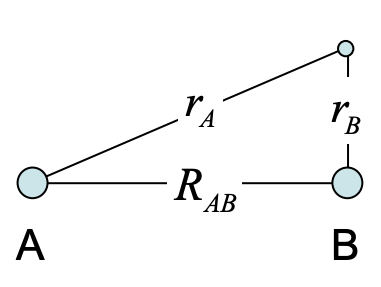
\includegraphics[width=40mm,scale=0.5]{h2_ion.png}
  \caption{\ce{H2+} with bond length $R_{AB}$}
\end{marginfigure}

\begin{equation}
  \hat{H} = \frac{-\hbar^2}{2m_e}\nabla^2_e + \frac{-\hbar^2}{2m_A}\nabla^2_A + \frac{-\hbar^2}{2m_B}\nabla^2_B + \frac{e^2}{4\pi\epsilon_0} \left( \frac{1}{R_{AB}} - \frac{1}{r_{A}} - \frac{1}{r_{B}} \right)
\end{equation}

\section{The Born-Oppenheimer Approximation}

\begin{definition}[Born-Oppenheimer Hamiltonian]
  As $\hat{T}_{n} = 0$,

  \begin{equation}
    \hat{H}_{\mathrm{BO}} = \left( \hat{T}_{e} + \hat{V}_{ee} + \hat{V}_{en} \right) + \hat{V}_{nn}
  \end{equation}
  where $\hat{V}_{nn}$ is the constant electrostatic repulsion between nuclei.
\end{definition}

For more information, see Appendix A.

\section{The Electronic Hamiltonian}

Through the Born-Oppenheimer approximation, we can write an \textit{electron-only version} of the Schrödinger equation. \marginnote[0.40cm]{The wavefunction and energy of the electrons depend on nuclear coordinates $R$.}
\begin{align*}
  \hat{H}_e \psi_e(\mathbf{r}_1, \mathbf{r}_2, \dots, \mathbf{r}_n) &= \left( \hat{T}_{e} + \hat{V}_{ee} + \hat{V}_{en} \right) \psi_e(\mathbf{r}_1, \mathbf{r}_2, \dots, \mathbf{r}_n) \\
      &= E(R) \psi_e(\mathbf{r}_1, \mathbf{r}_2, \dots, \mathbf{r}_n)
\end{align*}

\subsection{The Electronic Hamiltonian of \ce{H2+}}

The resulting \textit{electronic} Hamiltonian is much simpler,

\begin{equation}
  \hat{H}_e = \frac{-\hbar^2}{2m_e}\nabla^2_e + \frac{e^2}{4\pi\epsilon_0} \left( \frac{1}{R_{AB}} - \frac{1}{r_{A}} - \frac{1}{r_{B}} \right)
\end{equation}

As protons $A$ and $B$ have fixed positions in space, the \ce{H2+} cation now has a well-defined bond-length $R_{AB}$.

\section{Summary}

Here, we see that the \textbf{Born-Oppenheimer approximation} helps us to 1. simplify the Hamiltonian and 2. define molecular structure.


\section{Molecular Orbital Approximation}

At this point, we have nearly completed our introduction to quantum mechanics 
and we can investigate the electronic structure of molecules.

The Hamiltonian of \ce{H2+} is expressed as follows:

\begin{equation}
  \hat{H} = -\frac{1}{2}\nabla^2_r - \frac{\nabla^2_A}{2M_A}
\end{equation}

\subsection{The molecular orbitals of \ce{H2+}}

The \textbf{minimal basis set} is the smallest number of AOs required to describe the MO for a molecule. For \ce{H2+}
in its ground state, we require the $1\ce{s}$ orbital from each \ce{H} atom.

\begin{equation}
  \Psi(\ce{H2+}) = c_A [1\ce{s_}_A (\mathbf{r}_A)]+ c_B [1\ce{s_}_B (\mathbf{r}_B)]
\end{equation}

\textbf{A note on orbital coefficients.} The orbital coefficients $c$ provide us information
about electron density in a molecule. \textit{In this case,} \ce{H2+} is centrosymmetric. 
The electron is equally likely to be found aroun each nucleus A and B. Therefore, $c_A^2 = c_B^2 \rightarrow c_A = \pm c_B$.
$|c_A| > |c_B|$ would imply more electron density close
to $A$ than $B$.

\begin{example}[Molecular Orbitals of \ce{H2+}]

  \begin{equation}
    \psi(\ce{H2+}) = c_A[1\ce{s_}_A (\mathbf{r}_A) \pm 1\ce{s_}_B (\mathbf{r}_B)]
  \end{equation}

\begin{itemize}
  \item $1\ce{s_}_A (\mathbf{r}_A) + 1\ce{s_}_B (\mathbf{r}_B) \rightarrow$ constructive interference
  \item $1\ce{s_}_A (\mathbf{r}_A) - 1\ce{s_}_B (\mathbf{r}_B) \rightarrow$ destructive interference
\end{itemize}

\end{example}

\section{The Variational Principle}

\begin{theorem}[The Variational Theorem] $E_{\mathrm{avg}} > E_0$ for any function $\psi$. \marginnote{This
  makes physical sense, because energy of the ground state is, by definition, the lowest possible energy.}

  \begin{proof}
    Expand $\psi$ as a linear combination of unknown eigenstates $\phi_n$ of the Hamiltonian:
    \begin{equation*}
      \psi = \sum_n a_n \phi_n
    \end{equation*}
  \end{proof}
  
\end{theorem}

The variational method does two things for us. First, it gives us a way to compare two 
different wavefunctions and to show which one is closer to the wavefunction of the ground state. 

\section{Matrix Mechanics}

\begin{align}
  \hat{H} = \frac{-\hbar^2}{2m_e}\nabla^2_e + \frac{-\hbar^2}{2m_A}\nabla^2_A + \frac{-\hbar^2}{2m_B}\nabla^2_B \\
  + \frac{e^2}{4\pi\epsilon_0} \left( \frac{1}{R_{AB}} - \frac{1}{r_{A}} - \frac{1}{r_{B}} \right)
\end{align}

\section{Appendix A: The Born-Oppenheimer Approximation}

Nuclei are much heavier than electrons ($m_p / m_e = 1836$). Electrons appear to adjust their positions instantaneously to follow the slow nuclei.
As the wavefunction of the electrons ($\psi_e$) depends on the position of the nuclei, solving for $\psi_e$ with the nuclei fixed in space ($T_n = 0$) is a valid approximation.

\begin{enumerate}
  \item Separate the total wavefunction for a molecule (containing electrons and nuclei) into a product of two parts: an electronic part and a nuclear part.
  \item Treat the nuclei classically, as masses with well-defined positions, which can then be fixed in space to determine the electronic wavefunction.
\end{enumerate}

Much of our formal treatment of polyatomic electronic structure, such as \textbf{point groups}
which describe molecular symmetry, assume the fixed position of nuclei.

\subsection{Potenial Energy Surfaces}

The Born-Oppenheimer approximation defines a \textbf{potential energy surface} for our system.
A potential energy surface is a parametric function which describes the energy of electrons
as a function of nuclear coordinates. 

As nuclear positions are effectively fixed, we can specify their coordinates. The potential is the potential for nuclear motion that we have prevented.
Once we have the potential energy surface, 
\marginnote{Essentially treating vibrational and rotational motion with perturbation theory.}we can get vibrational and rotational energies. 

\subsection{Limitations}

The Born-Oppenheimer approximation is very reliable for ground \marginnote{Nuclear motion and energies give rise to discrete vibrational energy levels in IR spectroscopy, as well as zero-point energy.}electronic 
states, but it is less reliable for excited states. Nuclear wavefunctions
are important for understanding transitions between electronic states; we will have to consider vibrational transitions associated with them (see Document 3).

\section{Appendix B: Dirac Notation}

\begin{definition}[Dirac Notation]
  I'll figure this out sometime later.
  
\end{definition}

\bibliography{quantum}
\bibliographystyle{plainnat}



\end{document}
